\documentclass[10pt]{article}
\usepackage{fullpage}
\usepackage{graphicx}
\usepackage{amsmath}
\usepackage{amsmath} 

\author{Mirko van de Hoef}
\title{Deriving equations of motions of a double pendulum on a cart using the Lagrangian}
\date{\today}
\graphicspath{
    {img/}
}

\begin{document}

    \maketitle

    \section{Introduction}
    This file is made to document the simulation of a double pendulum on a cart using lagrangian mechanics. 
    In this file a double pendulum on a cart will be discussed.

    \section{The system}
    \begin{figure}{t}
        \centering
        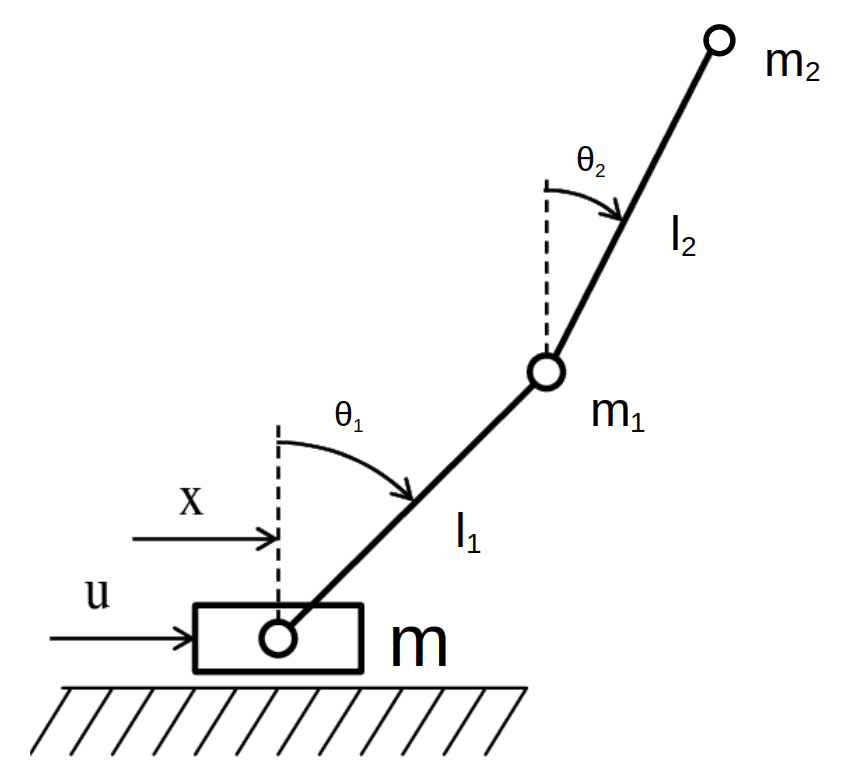
\includegraphics[width=5cm]{post-aRippol-02-pendulum_notations.png}
        \caption{The pendulum}
        \label{fig:system}
    \end{figure}
    
    Where in figure \ref{fig:system}: \\
    \begin{tabular}{@{}l l l@{}}
        & $M$: & Mass of the cart  [kg] \\
        & $m_1$: & Mass of the first pendulum  [kg] \\
        & $m_2$: & Mass of the second pendulum  [kg] \\
        & $\theta_1$: & Degrees first pendulum in reference to the cart [rad] \\
        & $\theta_2$: & Degrees second pendulum in reference to the cart [rad] \\
        & $\ell_1$: & Length of the first pendulum [m] \\
        & $\ell_2$: & Length of the second pendulum [m] \\
        & $x_c$: & Position of the cart [m] \\
    \end{tabular}
    

    \section{Lagrangian}
    Let the position and velocity of the pendulum be
    \begin{equation*}
    \begin{aligned}
        x_1 &= \ell_1 \sin(\theta_1) + x_c                                    & & \qquad \qquad & \dot x_1 &= \ell_1 \dot \theta_1 \cos(\theta_1) + \dot x \\
        y_1 &= -\ell_1 \cos(\theta_1)                                         & &  \quad \qquad & \dot y_1 &= \ell_1 \dot \theta_1 \sin(\theta_1)  \\
        x_2 &= \ell_1 \sin(\theta_1) + \ell_2 \sin(\theta_2) + x_c            & & \qquad \qquad & \dot x_2 &= \ell_1 \theta_1 \cos(\theta_1) + \ell_2 \dot \theta_2 \cos(\theta_2) + \dot x \\
        y_2 &= -\ell_1 \cos(\theta_1) - \ell_2 \cos(\theta_2)                 & &  \quad \qquad & \dot y_2 &= \ell_1 \dot \theta_1 \sin(\theta_1) + \ell_2 \dot \theta_2 \sin(\theta_2)  \\
    \end{aligned}
    \end{equation*}
    

    To derive the equations of motion, the Lagrangian (\ref{eq:lagrangian}) will be used.
    First, $T$, the kinetic energy of the system will be calculated.

    \begin{equation} \label{eq:lagrangian}
        \mathcal{L} = T - V
    \end{equation}

    \begin{equation}
        \begin{aligned} \label{eq:kinetic}
            T = &\frac{1}{2}  M  \dot x_c^2 + \frac{1}{2}  m_1(\dot x_1^2 + \dot y_1^2) + \frac{1}{2}m_2(\dot x_2^2 + \dot y_2^2) \\
            T = &\frac{1}{2}  M  \dot x_c^2 + \frac{1}{2}  m_1\left((\ell_1 \dot \theta_1 \cos(\theta_1) + \dot x_c)^2 + (\ell_1 \dot \theta_1 \sin(\theta_1))^2\right) \\
            &+ \frac{1}{2}  m_2\left((\ell_1 \dot \theta_1 \cos(\theta_1) + \dot x_c + \ell_2 \dot \theta_2\cos(\theta_2))^2 + (\ell_1 \dot \theta_2 \sin(\theta_1) + \ell_2\dot\theta_2\sin(\theta_2))^2\right)\\
            T = &\frac{1}{2} M\dot x_c^2 + \frac{1}{2}m_1(\dot x_c^2 + 2\ell_1\dot x_c \dot \theta_1 \cos(\theta_1) + \ell_1^2\dot\theta_1^2) + \frac{1}{2} m_2(...)\\
            T = &... + \frac{1}{2}m_2(\ell_1^2\dot\theta_1^2\cos(\theta_1)^2   \\
             &+ 2\ell_1\dot\theta_1\cos(\theta_2)\dot x_c + 2\ell_1\dot\theta_1\cos(\theta_1)\ell_2\dot\theta_2\cos(\theta_2)\\
             &+ \dot x_c^2 + 2\dot x_c \ell_2 \dot \theta_2 \cos(\theta_2) + \ell_2^2\dot\theta_2^2\cos(\theta_2)^2 \\
             &+\ell_1^2\dot\theta_1^2\sin(\theta_1)^2  +   2\ell_1\ell_2\dot\theta_1\dot\theta_2\sin(\theta_1)\sin(\theta_2) + \ell_2^2\dot\theta_2^2\sin(\theta_2)^2)\\
             T = &... + \frac{1}{2}m_2(\dot x_c^2 +\ell_1^2\dot\theta_1^2 + 2\ell_1\ell_2\dot\theta_1\dot\theta_2\cos(\theta_1 - \theta_2) + \ell_2^2\dot\theta_2^2     +      2\dot x_c(\ell_1\dot\theta_1\cos(\theta_1) + \ell_2\dot\theta_2\cos(\theta_2)))\\
             T = &\frac{1}{2}  (M + m_1 + m_2)  \dot x_c^2 + \frac{1}{2}(m_1 + m_2)\ell_1^2\dot\theta_1^2+ \frac{1}{2}m_2\ell_2^2\dot\theta_2^2\\
                 &+m_2\ell_1\ell_2\dot\theta_1\dot\theta_2\cos(\theta_1 - \theta_2)      +      (m_1 + m_2)\dot x_c\ell_1\dot\theta_1\cos(\theta_1) + m_2\dot x_c\ell_2\dot\theta_2\cos(\theta_2)\\
        \end{aligned}
    \end{equation}
    % \frac{1}{2}
    Then, for $V$, the potential energy of the system

    \begin{equation} \label{eq:potential}
        \begin{aligned}
        V &= m_1g(y_1) + m_2g(y_2)     \\
        V &= -m_1g\ell_1\cos(\theta_1) - m_2g(\ell_1\cos(\theta_1) +\ell_2\cos(\theta_2))\\
        V &= -(m_1+m_2)g\ell_1\cos(\theta_1) - m_2g\ell_2\cos(\theta_2)
        \end{aligned}
    \end{equation}
    
    Lastly, using (\ref{eq:kinetic}) and (\ref{eq:potential}) the 
    Lagrangian, $\mathcal{L}$, can be formulated
    
    \begin{equation} \label{eq:lagrangian_full}
        \begin{aligned}
            \mathcal{L} = &\frac{1}{2}  (M + m_1 + m_2)  \dot x_c^2 + \frac{1}{2}(m_1 + m_2)\ell_1^2\dot\theta_1^2+ \frac{1}{2}m_2\ell_2^2\dot\theta_2^2\\
            &+m_2\ell_1\ell_2\dot\theta_1\dot\theta_2\cos(\theta_1 - \theta_2)      +      (m_1 + m_2)\dot x_c\ell_1\dot\theta_1\cos(\theta_1) + m_2\dot x_c\ell_2\dot\theta_2\cos(\theta_2)\\
            & + (m_1 + m_2)g\ell_1\cos(\theta_1) + m_2g\ell_2\cos(\theta_2)
        \end{aligned}
    \end{equation}
    

    \pagebreak
    \section{Solve for $\ddot \theta_1$}

    Using the Lagrangian equation (\ref{eq:lagrangian_eq})
    \begin{equation} \label{eq:lagrangian_eq}
        \frac{d}{dt} \left(\frac{\partial \mathcal{L}}{\partial \dot q} \right) = 
        \frac{\partial \mathcal{L}}{\partial q}
    \end{equation}

    Substituting (\ref{eq:lagrangian_full}) in equation (\ref{eq:lagrangian_eq}) and solving for $\theta_1$ gives:
    \begin{equation} \label{eq: lagrange Step1}
        \frac{\partial \mathcal{L}}{\partial \dot\theta_1} = 
         (m_1 + m_2)\ell_1^2\dot\theta_1 + m_2\ell_1\ell_2\dot\theta_2\cos(\theta_1 - \theta_2) + (m_1+m_2)\dot x_c\ell_1\cos(\theta_1)
    \end{equation}

    \begin{equation} \label{eq: lagrange Step2}
        \begin{aligned}
        \frac{d}{dt} \left(\frac{\partial \mathcal{L}}{\partial \dot\theta_1}\right) =& 
         (m_1 + m_2)\ell_1^2\ddot\theta_1   +   m_2\ell_1\ell_2\ddot\theta_2\cos(\theta_1 - \theta_2)  -m_2\ell_1\ell_2\dot\theta_2\sin(\theta_1-\theta_2)(\dot\theta_1 - \dot\theta_2) \\
           & +   (m_1 +m_2)\ddot x_c\ell_1\cos(\theta_1) -(m_1 + m_2) \dot x_c\ell_1\sin(\theta_1)\dot\theta_1
        \end{aligned}
    \end{equation}

    
    \begin{equation} \label{eq: lagrange Step3}
        \frac{\partial \mathcal{L}}{\partial\theta_1} =
        -m_2\ell_1\ell_2\dot\theta_1\dot\theta_2\sin(\theta_1-\theta_2) 
        - (m_1 + m_2)g\ell_1\sin(\theta_1)
        -(m_1 +m_2)\dot x_c\ell_1\dot\theta_1\sin(\theta_1)
    \end{equation}

    Which give the following differential equation:

    \begin{equation}
        \begin{aligned}
            &(m_1 + m_2)\ell_1^2\ddot\theta_1   +   m_2\ell_1\ell_2\ddot\theta_2\cos(\theta_1 - \theta_2)  -m_2\ell_1\ell_2\dot\theta_2\sin(\theta_1-\theta_2)(\dot\theta_1 - \dot\theta_2)\\
            &+   (m_1 + m_2)\ddot x_c\ell_1\cos(\theta_1) - (m_1 + m_2) \dot x_c\ell_1\sin(\theta_1)\dot\theta_1 + m_2\ell_1\ell_2\dot\theta_1\dot\theta_2\sin(\theta_1-\theta_2) \\ 
            & + (m_1 + m_2)g\ell_1\sin(\theta_1) + (m_1 + m_2)\dot x_c\ell_1\dot\theta_1\sin(\theta_1) = 0
        \end{aligned}
    \end{equation}   


    Which simplifies to:

    \begin{equation}
        \begin{aligned}
            &(m_1 + m_2)\ell_1\ddot\theta_1   +   m_2\ell_2\ddot\theta_2\cos(\theta_1 - \theta_2)  +  m_2\ell_2\dot\theta_2^2\sin(\theta_1-\theta_2)\\
            &+   (m_1 + m_2)\ddot x_c\cos(\theta_1) + (m_1 + m_2)g\sin(\theta_1) = 0
        \end{aligned}
    \end{equation}  

    With the differential equation solved for $\ddot \theta_1$:
    \begin{equation}
        \begin{aligned}
            \frac{m_2\ell_2\ddot\theta_2\cos(\theta_1 - \theta_2)  +m_2\ell_2\dot\theta_2^2\sin(\theta_1-\theta_2)
            +   (m_1 + m_2)\ddot x_c\cos(\theta_1) + (m_1 + m_2)g\sin(\theta_1)}{-(m_1 + m_2)\ell_1} = \ddot \theta_1
        \end{aligned}
    \end{equation}  
    





    
    \pagebreak
    \section{Solve for $\ddot \theta_2$}

    Using the Lagrangian equation (\ref{eq:lagrangian_eq})
    \begin{equation} \label{eq:lagrangian_eq}
        \frac{d}{dt} \left(\frac{\partial \mathcal{L}}{\partial \dot q} \right) = 
        \frac{\partial \mathcal{L}}{\partial q}
    \end{equation}

    Substituting (\ref{eq:lagrangian_full}) in equation (\ref{eq:lagrangian_eq}) and solving for $\theta_1$ gives:

    \begin{equation} \label{eq: lagrange Step1}
        \frac{\partial \mathcal{L}}{\partial \dot\theta_1} = 
        m_2 \ell_1 \ell_2 \dot \theta_1 \cos(\theta_1 - \theta_2)
        + m_2\ell_2^2 \dot\theta_2 
        + m_2 \dot x_c \ell_2 \cos(\theta_2)
    \end{equation}

    \begin{equation} \label{eq: lagrange Step2}
        \begin{aligned}
        \frac{d}{dt} \left(\frac{\partial \mathcal{L}}{\partial \dot\theta_1}\right) &= 
        m_2 \ell_1 \ell_2 \ddot \theta_1 \cos(\theta_1 - \theta_2) - m_2 \ell_1 \ell_2 \dot \theta_1 \sin(\theta_1 - \theta_2)(\dot \theta_1 - \dot \theta_2)\\
        &+m_2\ell_2^2 \ddot \theta_2 + m_2 \ddot x_c \ell_2 \cos(\theta_2) - m_2 \dot x_c \ell_2 \sin(\theta_2)\dot\theta_2
        \end{aligned}
    \end{equation}

    
    \begin{equation} \label{eq: lagrange Step3}
        \frac{\partial \mathcal{L}}{\partial\theta_1} =
        -m_2 \ell_1 \ell_2 \dot \theta_1 \dot\theta_2\sin(\theta_1-\theta_2)
        -m_2\dot x_c \dot \theta_2 \ell_2 \sin(\theta_2)
        -m_2g\ell_2\sin(\theta_2)
        \end{equation}

    Which give the following differential equation:

    \begin{equation}
        \begin{aligned}
                &m_2 \ell_1 \ell_2 \ddot \theta_1 \cos(\theta_1 - \theta_2) - m_2 \ell_1 \ell_2 \dot \theta_1 \sin(\theta_1 - \theta_2)(\dot \theta_1 - \dot \theta_2)\\
                &+m_2\ell_2^2 \ddot \theta_2 + m_2 \ddot x_c \ell_2 \cos(\theta_2) - m_2 \dot x_c \ell_2 \sin(\theta_2)\dot\theta_2 + m_2 \ell_1 \ell_2 \dot \theta_1 \dot\theta_2\sin(\theta_1 - \theta_2)\\
                &+m_2\dot x_c \dot \theta_2 \ell_2 \sin(\theta_2)+m_2g\ell_2\sin(\theta_2) = 0
        \end{aligned}
    \end{equation}   


    Which simplifies to:

    \begin{equation}
        \begin{aligned}
            &m_2\ell_2 \ddot \theta_2 + m_2 \ell_1  \ddot \theta_1 \cos(\theta_1 - \theta_2) - m_2 \ell_1\dot \theta_1^2 \sin(\theta_1 - \theta_2)+ m_2 \ddot x_c  \cos(\theta_2) +m_2g\sin(\theta_2) =0
        \end{aligned}
    \end{equation}  

    With the differential equation solved for $\ddot \theta_1$:
    \begin{equation}
        \begin{aligned}
            \frac{m_2 \ell_1  \ddot \theta_1 \cos(\theta_1 - \theta_2) - m_2 \ell_1\dot \theta_1^2 \sin(\theta_1 - \theta_2)+ m_2 \ddot x_c  \cos(\theta_2) +m_2g\sin(\theta_2)}{-m_2 \ell_2} = \ddot \theta_2
        \end{aligned}
    \end{equation}  



    \pagebreak
    \section{Solve for $\ddot x_c$}
    Using the Lagrangian equation (\ref{eq:lagrangian_eq})
    \begin{equation} \label{eq:lagrangian_eq}
        \frac{d}{dt} \left(\frac{\partial \mathcal{L}}{\partial \dot q} \right) = 
        \frac{\partial \mathcal{L}}{\partial q}
    \end{equation}

    Substituting (\ref{eq:lagrangian_full}) in equation (\ref{eq:lagrangian_eq}) and solving for $\theta_1$ gives:

    \begin{equation} \label{eq: lagrange Step1}
        \frac{\partial \mathcal{L}}{\partial \dot x_c} = (M + m_1 + m_2)\dot x_c + (m_1 + m_2)\ell_1\dot\theta_1\cos(\theta_1) + m_2\ell_2\dot\theta_2\cos(\theta_2)
    \end{equation}

    \begin{equation} \label{eq: lagrange Step2}
        \begin{aligned}
        \frac{d}{dt} \left(\frac{\partial \mathcal{L}}{\partial \dot x_c}\right) &= (M + m_1 + m_2)\ddot x_c +  (m_1 + m_2)\ell_1\ddot\theta_1\cos(\theta_1)\\
         &- (m_1 + m_2)\ell_1\dot\theta_1^2\sin(\theta_1) + m_2\ell_2\ddot\theta_2\cos(\theta_2) - m_2\ell_2\dot\theta_2^2\sin(\theta_2)
        \end{aligned}
    \end{equation}

    
    \begin{equation} \label{eq: lagrange Step3}
        \frac{\partial \mathcal{L}}{\partial x_c} = 0
        \end{equation}

    Which give the following differential equation:

    \begin{equation}
        \begin{aligned}
            &(M + m_1 + m_2)\ddot x_c +  (m_1 + m_2)\ell_1\ddot\theta_1\cos(\theta_1)\\
            &- (m_1 + m_2)\ell_1\dot\theta_1^2\sin(\theta_1) + m_2\ell_2\ddot\theta_2\cos(\theta_2) - m_2\ell_2\dot\theta_2^2\sin(\theta_2)  = 0      
        \end{aligned}
    \end{equation}   

    With the differential equation solved for $\ddot x_c$:
    \begin{equation}
        \begin{aligned}
            \frac{(m_1 + m_2)\ell_1\ddot\theta_1\cos(\theta_1) - (m_1 + m_2)\ell_1\dot\theta_1^2\sin(\theta_1) + m_2\ell_2\ddot\theta_2\cos(\theta_2) - m_2\ell_2\dot\theta_2^2\sin(\theta_2)}{-M+m_1+m_2} = \ddot x_c
        \end{aligned}
    \end{equation}  




    \pagebreak
    \section{Liniearize using small angle approxiomation for: $\ddot x_c, \ddot \theta_1, \ddot \theta_2$}

    \begin{equation}
        \begin{aligned}
            &(M+m_1+m_2)\ddot x_c + (m_1+m_2)\ell_1\ddot\theta_1 + m_2\ell_2\ddot\theta_2\    = F
        \end{aligned}   
    \end{equation}

    \begin{equation}
        \begin{aligned}
            (m_1 + m_2)\ell_1\ddot \theta_1 + m_2\ell_2\ddot\theta_2
            +   (m_1 +m_2)\ddot x_c - (m_1 + m_2)g\theta_1 = 0 
        \end{aligned}   
    \end{equation}

    \begin{equation}
        \begin{aligned}
            m_2\ell_2\ddot \theta_2 + m_2\ell_1  \ddot \theta_1 +  m_2\ddot x_c -m_2g\theta_2 = 0\\
        \end{aligned}   
    \end{equation}
    




    Or in matrix form:
    \begin{equation}
        \begin{bmatrix}
            (M+m_1+m_2) & (m_1+m_2)\ell_1         & m_2\ell_2\\
            (m_1 +m_2)     & (m_1+m_2)\ell_1   & m_2\ell_2\\
            m_2      & m_2\ell_1            &  m_2\ell_2
        \end{bmatrix}
        \begin{bmatrix}
            \ddot x_c\\
            \ddot \theta_1\\
            \ddot \theta_2\\
        \end{bmatrix}
        +
        \begin{bmatrix}
            0&0&0\\
            0&-(m_1 +m_2)g&0\\
            0&0&-g
        \end{bmatrix}
        \begin{bmatrix}
            x_c\\
            \theta_1\\
            \theta_2
        \end{bmatrix}
        =
        \begin{bmatrix}
            F\\
            0\\
            0
        \end{bmatrix}
    \end{equation}

    With state vector equalling:
    \begin{equation}
        X=
        \begin{bmatrix}
            x_c\\
            \theta_1\\
            \theta_2\\
            \dot x_c\\
            \dot \theta_1\\
            \dot \theta_2
        \end{bmatrix}   
        \qquad\text{or}\qquad\dot X=
        \begin{bmatrix}
            \dot x_c\\
            \dot \theta_1\\
            \dot \theta_2\\
            \ddot x_c\\
            \ddot \theta_1\\
            \ddot \theta_2
        \end{bmatrix}   
    \end{equation}

    Now write the second-order into the first-order form: $M \dot X + NX = F$:

    \begin{equation}
        \resizebox{.9\textwidth}{!}{$
        M=
        \begin{bmatrix}
            1&0&0&0&0&0\\
            0&1&0&0&0&0\\
            0&0&1&0&0&0\\
            0&0&0&(M+m_2+m_1) & (m_1+m_2)\ell_1         & m_2\ell_2\\
            0&0&0&(m_1 + m_2)      & (m_1+m_2)\ell_1            &  m_2\ell_2\\
            0&0&0&m2     & m_2\ell_1   & m_2\ell_2
        \end{bmatrix}
        ,N =
        \begin{bmatrix}
            0&0&0&1&0&0\\
            0&0&0&0&1&0\\
            0&0&0&0&0&1\\
            0&0&0&0&0&0\\
            0&(m_1 +m_2)g&0&0&0&0\\
            0&0& g &0&0&0
        \end{bmatrix}
        ,F=
        \begin{bmatrix}
            0\\
            0\\
            0\\
            1\\
            0\\
            0\\
        \end{bmatrix}$}
    \end{equation}

    Using the following formula for calculating the A and B matrix for the state space:
    \begin{equation}
        A = M^{-1}N, B = M^{-1}F (\text{voeg bron in}) 
    \end{equation}
    Resulting in the following matrices:


    \begin{equation*}
        A = 
        \begin{bmatrix}
            0 & 0 & 0 & 1 & 0 & 0 \\
            0 & 0 & 0 & 0 & 1 & 0 \\
            0 & 0 & 0 & 0 & 0 & 1 \\
            0 & \frac{-g(m_1 + m_2)}{M} & 0 & 0 & 0 & 0 \\
            0 & \frac{g(M + m_1)(m_1 + m_2)}{(Ml_1m_1)} & \frac{-g m_2}{(l_1 m_1)} & 0 & 0 & 0 \\
            0 & \frac{-g(m_1 + m_2)}{(l_2 m_1)} & \frac{g(m_1 + m_2)}{(l_2 m_1)} & 0 & 0 & 0 \\
        \end{bmatrix}
        ,         B = 
        \begin{bmatrix}
            0 \\
            0 \\
            0 \\
            1/M \\
            -1/Ml_1 \\
            0 \\
        \end{bmatrix}
    \end{equation*}
    
    \begin{equation*}
        C = 
        \begin{bmatrix}
            1&0&0&0&0&0\\
            0&1&0&0&0&0\\
            0&0&1&0&0&0\\
        \end{bmatrix}
        \qquad D= 
        \begin{bmatrix}
            0\\
            0\\
            0\\
        \end{bmatrix}
    \end{equation*}


\end{document}






















   % \begin{equation}
    %     \begin{aligned}
    %         x_1 = x_c               \qquad \dot x_1 =...\\
    %         x_2 = \dot x_c          \qquad \dot x_2 =...\\
    %         x_3 = \theta_1          \qquad \dot x_3 =...\\
    %         x_4 = \dot \theta_1     \qquad \dot x_4 =...\\
    %         x_5 = \theta_2          \qquad \dot x_5 =...\\
    %         x_6 = \dot \theta_2     \qquad \dot x_6 =...\\      
    %     \end{aligned}
    % \end{equation}

    % \begin{equation}
    %     \begin{bmatrix}
    %         \dot x_1\\
    %         \dot x_2\\
    %         \dot x_3\\
    %         \dot x_4\\
    %         \dot x_5\\
    %         \dot x_6\\
    %     \end{bmatrix}
    %     =
    %     \begin{bmatrix}
    %         0&1&0&0&0&0\\
    %         0&0&0&\frac{-m_2\ell_1}{M+m_1}&0&\frac{m_2\ell_2}{M+m_1}\\
    %         0&0&0&1&0&0\\
    %         0&\frac{-m_2}{(m_1+m_2)\ell_1}&\frac{g}{\ell_1}&0&0&\frac{-m_2\ell_1}{(m_1+m_2)\ell_1}\\
    %         0&0&0&0&0&1\\
    %         0&\frac{1}{\ell_2}&0&\frac{-\ell_1}{\ell_2}&\frac{-g}{\ell_2}&0
    %     \end{bmatrix}
    %     \begin{bmatrix}
    %         x_1\\
    %         x_2\\
    %         x_3\\
    %         x_4\\
    %         x_5\\
    %         x_6
    %     \end{bmatrix}
    %     +
    %     \begin{bmatrix}
    %         0\\
    %         \frac{1}{M+m_1}\\
    %         0\\
    %         0\\
    %         0\\
    %         0\\
    %     \end{bmatrix}
    %     F
    % \end{equation}
    
    % \begin{equation}
    %     \begin{aligned}
    %         &\frac{m_2\ell_1 m_2\ell_2\ddot\theta_2 + m_2\ddot x_c + (m_1 + m_2)g\theta_1 - m_2\ell_2\ell_1  \ddot \theta_1 -  \ddot x_c +g\theta_2 - m_2\ell_2\dot\theta_2^2}{-M+m_1*(-(m_1 + m_2)\ell_1) * (-\ell_2)} = \ddot x_c
    %     \end{aligned}   
    % \end{equation}  

    

    % Or in a second-order derivative matrix form: $\ddot X$ = A$\dot X$ + B$X$, where:
    % \begin{equation}
    %     X=
    %     \begin{bmatrix}
    %         x_c\\
    %         \theta_1\\
    %         \theta_2\\
    %         \dot x_c\\
    %         \dot \theta_1\\
    %         \dot \theta_2
    %     \end{bmatrix}         
    % \end{equation}
